\section{Scaling Laws for Fixed Latent Design}
\begin{figure}
    \centering
    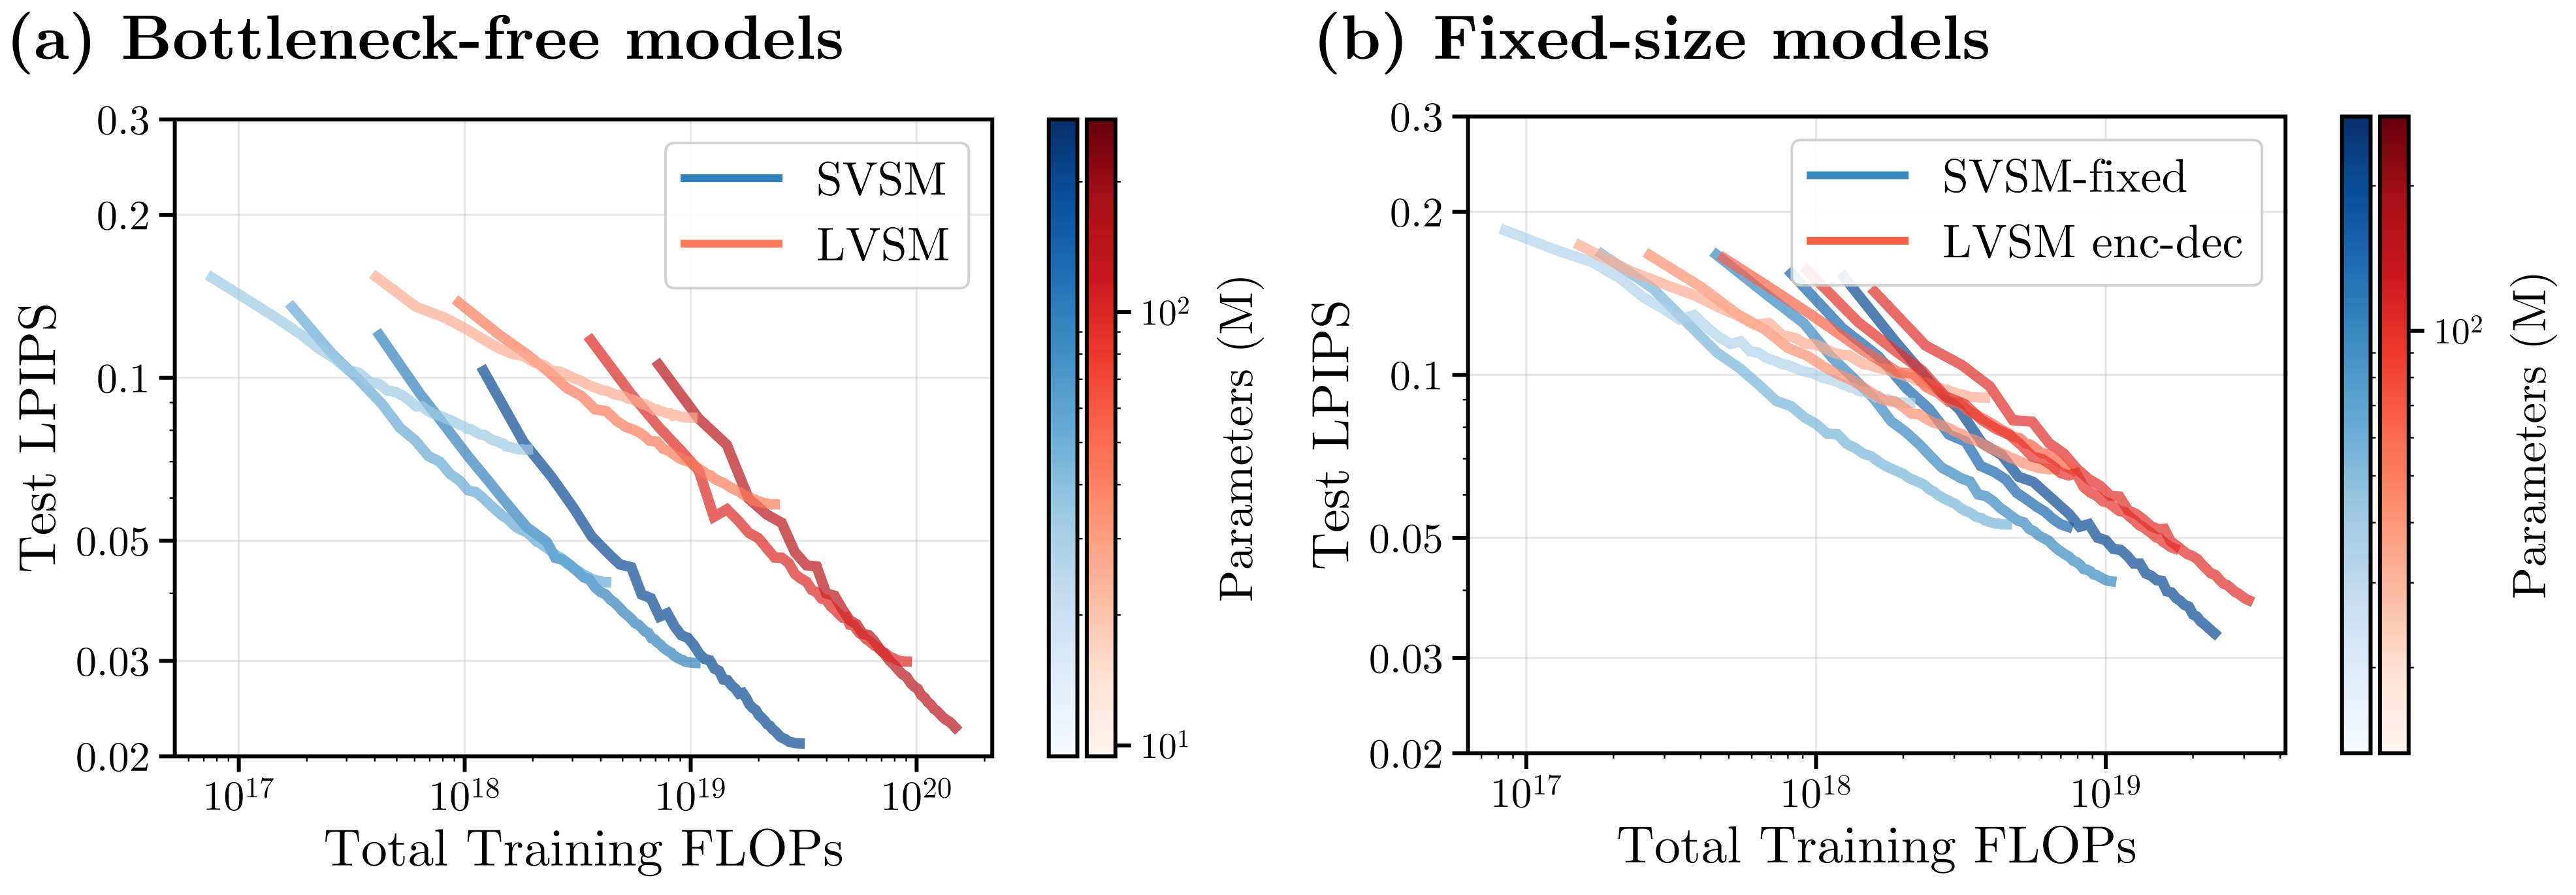
\includegraphics[width=\linewidth]{images/obj_scaling_final_fixed.png}
    \caption{\textbf{Fixed-size Latent Scaling Experiments.} Conducted on Objaverse~\cite{objaverse}. \textbf{(a)} For $V_C{=}8$, SVSM and LVSM decoder-only scale equally while SVSM's frontier is shifted by $5\times$ on the compute axis. \textbf{(b)} When a fixed latent bottleneck is used, SVSM-fixed and LVSM encoder-decoder scale equally, but significantly worse than the unbottlenecked designs. SVSM again maintains a superior pareto frontier.}
    \label{fig:obj_scale}
\end{figure}

\paragraph{Analysis Setup.} Lastly, we check both the scaling laws and the design space of view synthesis models with a fixed-size scene representation. This design has favorable rendering speeds for large context lengths, though it does not have favorable training compute as the encoder is still quadratic in the context length. For training and evaluation, we use Objaverse~\citep{objaverse}, with 8 context views (where the benefit of having a fixed latent starts to appear at inference time). We compare two designs: LVSM Encoder-Decoder and SVSM-fixed, which follows the same design of a unidirectional decoder but instead decodes off of a fixed latent. Both models utilize PRoPE with identity pose on the scene representation. We use $V_T = 8$ and scene batch size $64$ for an effective batch size of $512$ for all experiments. All other settings follow those described in Sec.~\ref{sec:scaling-two-view} and \suppref{supp:exp-details}.

\paragraph{SVSM-Fixed Matches LVSM Scaling, but Both Scale Poorly.} As shown in Fig.~\ref{fig:obj_scale}b, SVSM with a fixed latent and the LVSM encoder–decoder exhibit similar scaling behavior. However, SVSM-fixed consistently requires less compute to achieve the same performance, maintaining a Pareto advantage. This indicates that our unidirectional decoder remains more compute-efficient even when a fixed latent bottleneck is imposed, which is desirable when amortized rendering is required. Nevertheless, comparing to Fig.~\ref{fig:obj_scale}a makes clear that both fixed-latent designs scale substantially worse than their bottleneck-free counterparts.